\chapter{Measurements}
Several measurement campaigns were done to characterize the system.
A number of measurements were done at different solenoid tilt
angles, to estimate the effect of tilt-swing misalignment on 
the peak shifts of coils. Maps with all 21 coils
were done at a number of angles, as well as repeated measurements
for accuracy estimation. A number of procedures had to be developed
in order to make the measurements repeatable. 

\section{The Fluxmeter Alignment Procedure}
An alignment procedure was developed for the fluxmeter, so that
measurements could be taken in an aligned, almost ideal case
or with a desired tilt-swing angle between the solenoid and the magnet.

Aligning the fluxmeter to a desired angle is an iterative procedure.
First, the laser tracker is used to sample the fluxmeter positions
as it is pulled through the tube. These samples are then fitted to
a line in three dimensional space, as in figure \ref{fig:geomfit}.

\begin{figure}[!h]
    \centering
    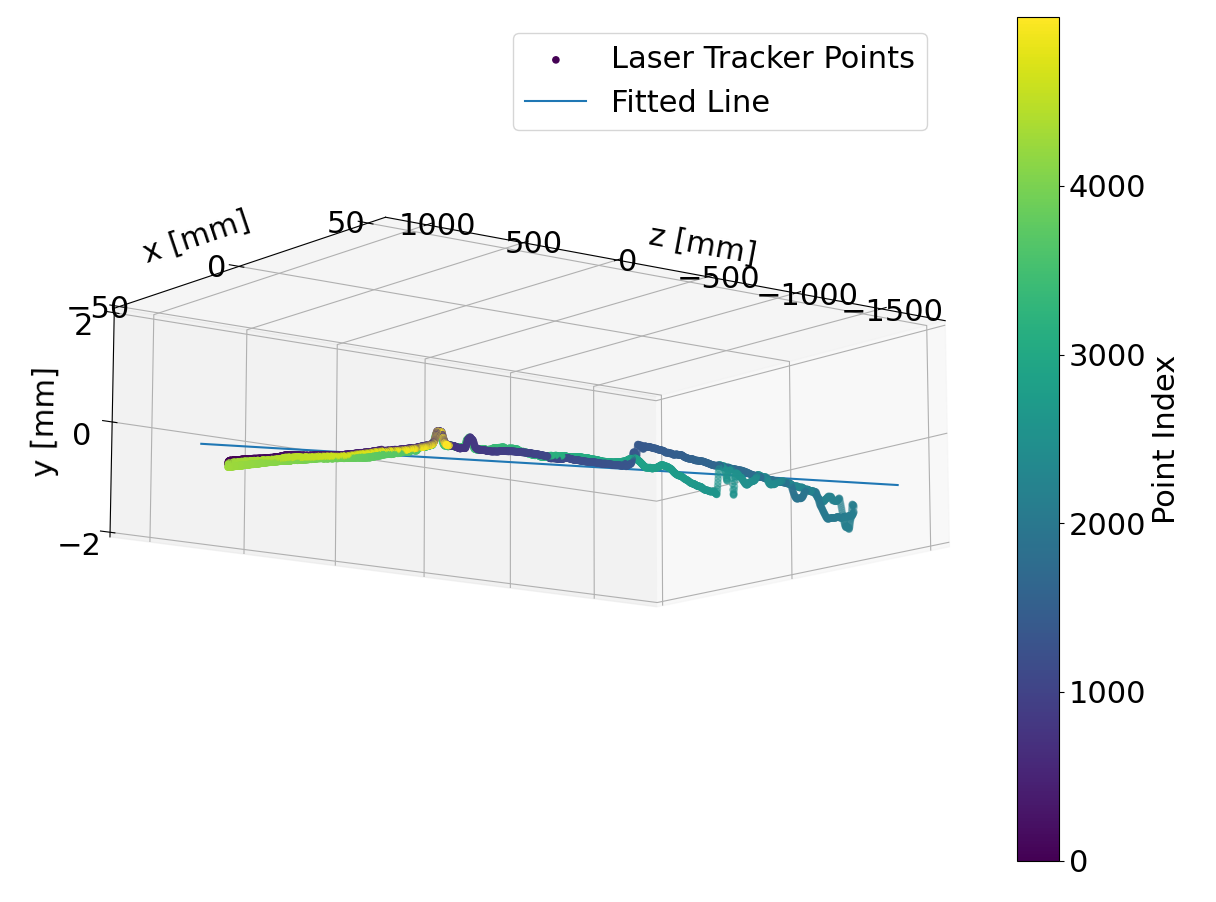
\includegraphics[width=0.8\linewidth]{figs/geomfit}
    \caption{Measured fluxmeter positions along with a line
    fit. The fluxmeter tube is tilted by $30$ mrad around the y axis.}
    \label{fig:geomfit}
\end{figure}

The intersections between the fluxmeter path line and the 
planes $z = z_{Back}$, $z = z_{Front}$ are then found, where
$z_{Back}$ and $z_{Front}$ are the z positions where the tube clamps
are located.

\begin{figure}[!h]
    \centering
    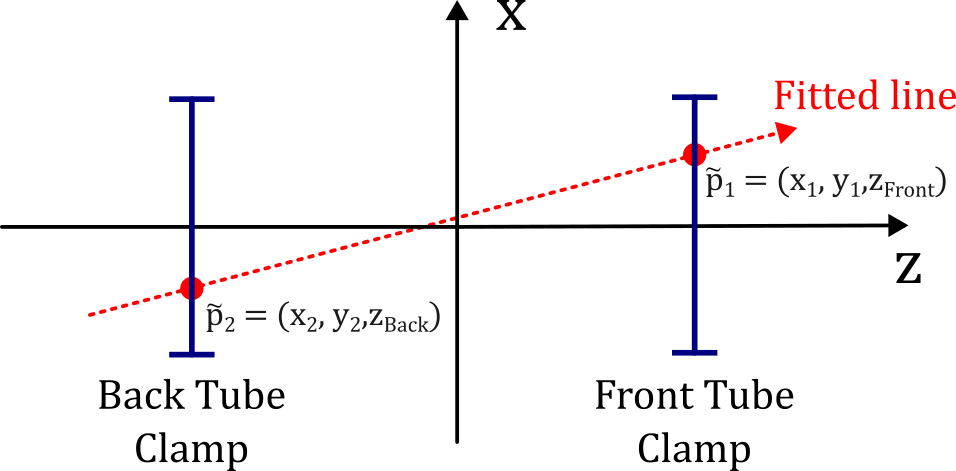
\includegraphics[width=0.8\linewidth]{figs/alignment}
    \caption{The fluxmeter path and its intersection points with
    the tube clamps.}
    \label{fig:alignment}
\end{figure}


\section{Solenoidal Field Maps}
\section{The Magnet-Magnetometer Yaw Angle Peak Shift}